\documentclass[tikz]{standalone}
\usepackage[utf8x]{inputenc}
\usepackage{tikz}
\usetikzlibrary{patterns}
\begin{document}
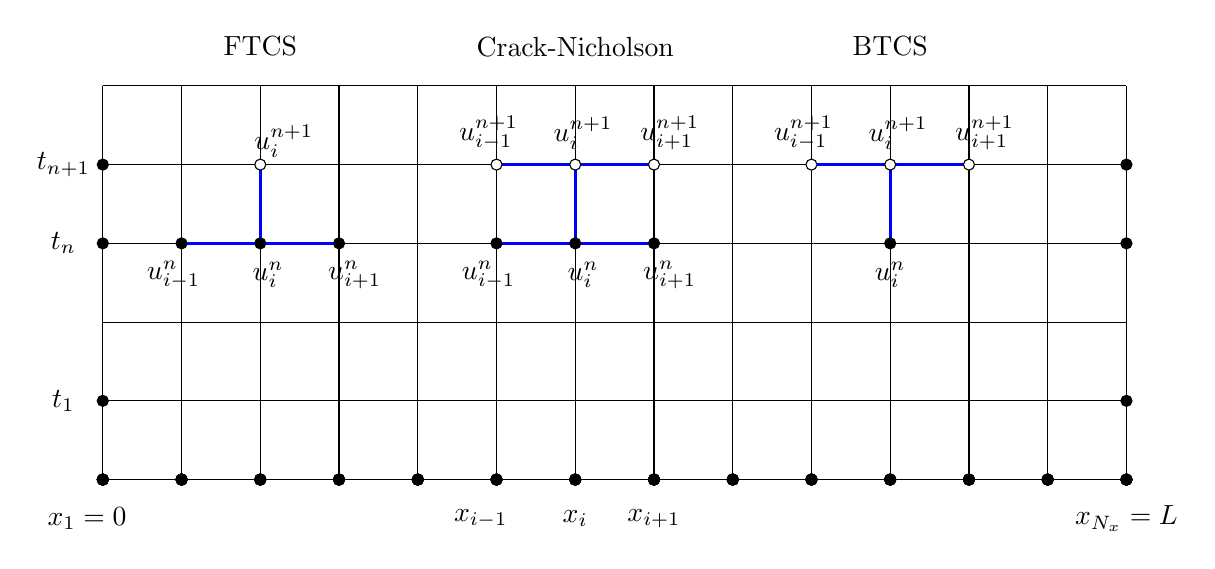
\begin{tikzpicture}[font=\normalsize]

	\foreach \x in {0, 1, 2, 3, 4, 5, 6, 7, 8 , 9, 10, 11, 12, 13}
		\foreach  \y in {0, 1, 2, 3, 4, 5}
			{
				\draw (\x, 0) -- (\x, 5);
				\draw (0, \y) -- (13, \y);
				\draw [fill] (\x, 0) circle (2pt);
				
			}

	\foreach \x in {0, 13}
		\foreach \y in {1, 3, 4}
			{
				\draw [fill] (\x, \y) circle (2pt);
			}
	
	\draw (-0.2, -0.5) node {$x_{1} = 0$};
	\draw (4.8, -0.5) node {$x_{i-1}$};
	\draw (6, -0.5) node {$x_{i}$};
	\draw (7, -0.5) node {$x_{i+1}$};
	\draw (13, -0.5) node {$x_{N_{x}} = L$};

	\draw (-0.5, 1) node {$t_{1}$};
	\draw (-0.5, 3) node {$t_{n}$};
	\draw (-0.5, 4) node {$t_{n+1}$};

	\draw [very thick, color=blue] (1, 3) -- (2, 3) -- (3, 3);
	\draw [very thick, color=blue] (2, 3) -- (2, 4);
	\draw [fill=white] (2, 4) circle (2pt);

	\foreach \x in {1, 2, 3}
		\draw [fill] (\x, 3) circle (2pt);

	\draw (0.9, 2.6) node {$u_{i-1}^{n}$};
	\draw (2.1, 2.6) node {$u_{i}^{n}$};
	\draw (3.2, 2.6) node {$u_{i+1}^{n}$};
	\draw (2.3, 4.3) node {$u_{i}^{n+1}$};

	\foreach \y in {3, 4}
		\draw [very thick, color=blue] (5, \y) -- (6, \y) -- (7, \y);
		
	\draw [very thick, color=blue] (6, 3) -- (6, 4);

	\foreach \x in {5, 6, 7}
		{
			\draw [fill] (\x, 3) circle (2pt);
			\draw [fill=white] (\x, 4) circle (2pt);
		}
	\draw (4.9, 2.6) node {$u_{i-1}^{n}$};
	\draw (6.1, 2.6) node {$u_{i}^{n}$};
	\draw (7.2, 2.6) node {$u_{i+1}^{n}$};

	\draw (4.9, 4.4) node {$u_{i-1}^{n+1}$};
	\draw (6.1, 4.4) node {$u_{i}^{n+1}$};
	\draw (7.2, 4.4) node {$u_{i+1}^{n+1}$};

	\draw [very thick, color=blue] (9, 4) -- (10, 4) -- (11, 4);
	\draw [very thick, color=blue] (10, 4)  -- (10, 3);
	\draw [fill] (10, 3) circle (2pt);

	\foreach \x in {9, 10, 11}
		\draw [fill=white] (\x, 4) circle (2pt);

	\draw (10, 2.6) node {$u_{i}^{n}$};
	\draw (8.9, 4.4) node {$u_{i-1}^{n+1}$};
	\draw (10.1, 4.4) node {$u_{i}^{n+1}$};
	\draw (11.2, 4.4) node {$u_{i+1}^{n+1}$};

	\draw (2, 5.5) node {FTCS};
	\draw (6, 5.5) node {Crack-Nicholson};
	\draw (10, 5.5) node {BTCS};
\end{tikzpicture}
\end{document}